\textbf{جدول
\lr{t}
در ادامه آمده است.}

اداره هواشناسی یک شهر، ۴ دستگاه سنجش آلودگی هوا را در یک منطقه قرار داده است. فرض کنید شاخص آلودگی هوا در این منطقه ثابت است اما این دستگاه‌ها دقیق نیستند و شاخص را با کمی نویز گزارش می‌دهند. در یک روز نسبتا آلوده، مقادیر گزارش شده توسط این ۴ دستگاه به شرح زیر است.
$$152, 148, 153, 153$$

\subsection*{الف}
با کمک داده‌های جمع آوری شده، یک بازه اطمینان ۹۵ درصد برای شاخص آلودگی هوا در آن ایستگاه ارائه دهید.

\subsection*{ب}
در صورتی که شاخص آلودگی هوا از ۱۵۰ بیشتر باشد، هوا در شرایط ناسالم برای تمامی گروه‌ها قرار می‌گیرد. عده‌ای از دانشمندان معتقدند که میانگین شاخص آلودگی ۱۵۰ بوده بنابراین هوای این منطقه ناسالم نیست، در حالی که عده‌ی دیگری معتقند میانگین شاخص آلودگی به طور معنی‌داری از ۱۵۰ بیشتر بوده و هوا ناسالم است. برای بررسی این افراد یک آزمون فرض طراحی کنید. فرض صفر و فرض دیگر این آزمون را بیان کرده و سپس مشخص کنید آیا با سطح اهمیت 
$0.05$
می‌توان فرض صفر را رد کرد یا خیر.

\subsection*{پ}
برای کاهش خطای نوع اول، باید سطح اهمیت را افزایش دهیم یا کاهش؟ برای کاهش خطای نوع دوم چه طور؟

\begin{figure}[H]
    \centering
    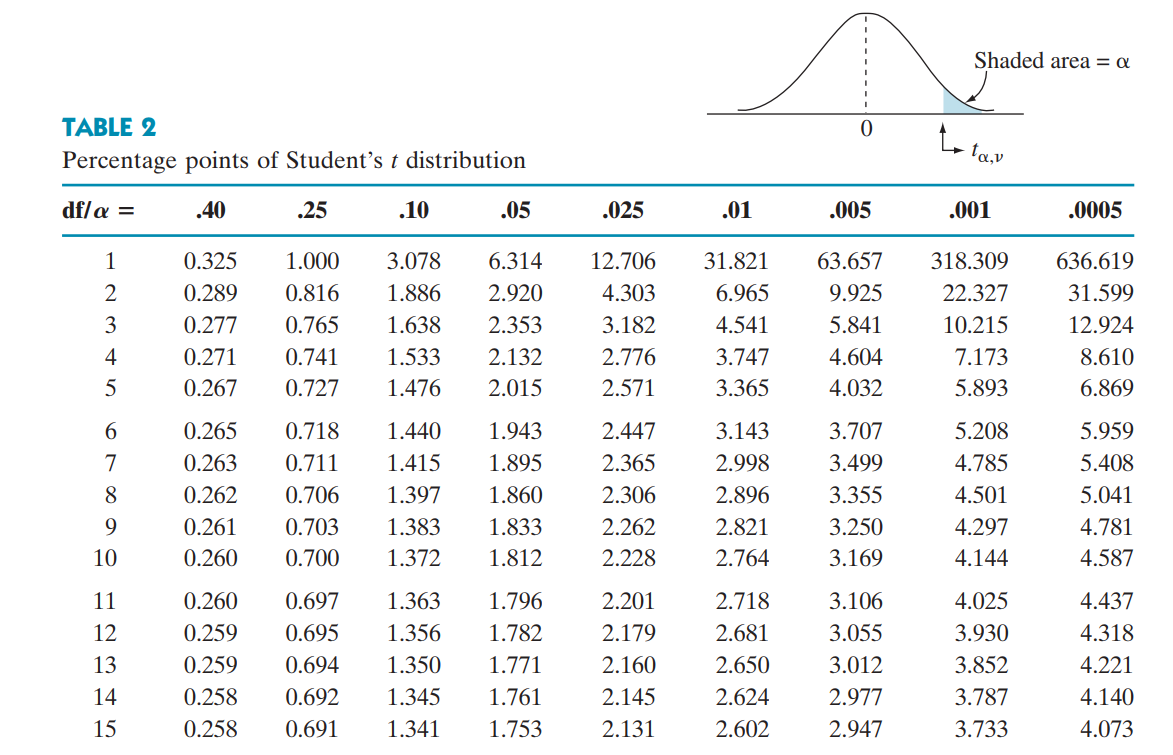
\includegraphics[width=7in,height = 5in]{tStudent}
\end{figure}